\documentclass[conference]{IEEEtran}
\IEEEoverridecommandlockouts
% The preceding line is only needed to identify funding in the first footnote. If that is unneeded, please comment it out.
\usepackage[margin=0.25in]{geometry}
\usepackage{cite}
\usepackage{amsmath,amssymb,amsfonts}
\usepackage{algorithmic}
\usepackage{graphicx}
\usepackage{textcomp}
\usepackage{xcolor}
\usepackage{hyperref}
\def\BibTeX{{\rm B\kern-.05em{\sc i\kern-.025em b}\kern-.08em
    T\kern-.1667em\lower.7ex\hbox{E}\kern-.125emX}}
\begin{document}

\title{}

\author{\IEEEauthorblockN{} }

\maketitle

\section{Intro}

\subsection{Difference between AI, ML, and DL}

\begin{itemize}
    \item AI: Membuat algoritma yang dapat melakukan tugas yang biasanya memerlukan kecerdasan manusia tanpa dibuat secara eksplisit
    \item Machine Learning: Membuat algoritma yang dapat belajar dari data
    \item Deep Learning: Membuat algoritma yang dapat belajar dari data dengan menggunakan \textit{neural network} yang memiliki banyak lapisan
\end{itemize}

\subsection{Difference in AI Methods}

\begin{itemize}
    \item Supervised Learning: Algoritma belajar dari data yang sudah diberikan label
    \item Unsupervised Learning: Algoritma belajar dari data yang tidak diberikan label
    \item Reinforcement Learning: Algoritma belajar dari interaksi dengan lingkungan dan mendapatkan \textit{reward} atau \textit{penalty} dari tindakan yang dilakukan
\end{itemize}

\subsection{AI Pipeline}

CRISP-DM: \textit{Cross Industry Standard Process for Data Mining}

% % image
% \begin{figure}[htbp]
%     \centerline{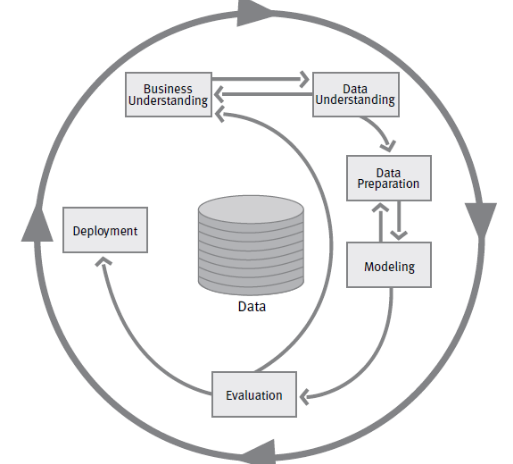
\includegraphics[width=0.2\textwidth]{crisp.png}}
% \end{figure}

\begin{itemize}
    \item Business Understanding: Memahami tujuan dari proyek
    \item Data Understanding: Memahami data yang digunakan
    \item Data Preparation: Menyiapkan data yang digunakan
    \item Modeling: Membuat model dari data yang sudah disiapkan
    \item Evaluation: Mengevaluasi model yang sudah dibuat
    \item Deployment: Menerapkan model yang sudah dibuat
\end{itemize}

% Other pipeline
% \begin{figure}[htbp]
%     \centerline{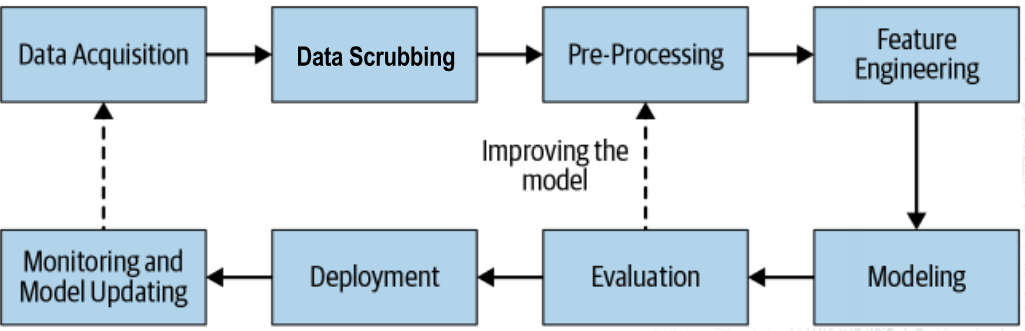
\includegraphics[width=0.3\textwidth]{pipeline.png}}
% \end{figure}

\section{Data Preprocessing}

\subsection{Data Scrubbing}
\begin{itemize}
    \item Identifikasi data yang hilang
    \item Menghilangkan outlier
    \item Memperbaiki format
    \item Menghilangkan data duplikat
    \item Menangani data yang tidak konsisten
\end{itemize}

\subsection{Feature Engineering}
\begin{itemize}
    \item Feature Selection: Memilih fitur yang penting saja
    \item Feature Reduction: Mengurangi fitur yang tidak penting, dengan contoh menggabungkan fitur yang memiliki korelasi tinggi (jumlah produk A, B, C seluruhnya dijumlah menjadi fitur baru)
    \item Row Compression: Menggabungkan beberapa baris data menjadi satu baris data, contoh ada item instance untuk tiger, lion, dan bear, maka dijadikan satu baris data saja
\end{itemize}

\subsection{Data Representation}
\begin{itemize}
    \item One-Hot Encoding: Mengubah data kategorikal menjadi data numerik, dengan setiap kategori menjadi kolom baru dengan nilai 0 atau 1
    \item Binning: Mengubah data numerik menjadi data kategorikal, dengan mengelompokkan data numerik menjadi beberapa kelompok
    \item Normalization: Mengubah data numerik menjadi data yang memiliki rentang nilai yang sama
\end{itemize}

\section{Model}

\subsection{Training}

\begin{itemize}
    \item Split validation: Memisahkan data menjadi data training dan data validasi (70/30 atau 80/20), perlu randomisasi data sebelum memisahkan
    \item Cross validation: Memisahkan data menjadi beberapa bagian, dan melakukan training dan validasi sebanyak bagian yang ada
    \begin{itemize}
        \item K-Fold Cross Validation: Memisahkan data menjadi K bucket, dan melakukan training dan validasi sebanyak K kali, dengan setiap bucket menjadi data tes satu kali dengan bucket lainnya menjadi data training
        \item Exhausive Cross Validation: Memisahkan data menjadi semua kemungkinan kombinasi training dan validasi
    \end{itemize}
    \item Jumlah sampel perlu \(\ge 10 \times \text{feature}\)
\end{itemize}

\subsection{Model Evaluation/Post Analyss}

Menentukan model baik

\begin{itemize}
    \item Generalazation Capability: Model dapat memprediksi data yang belum pernah dilihat sebelumnya
    \item Interpretability: Model dapat dijelaskan dengan mudah
    \item Prediction speed: Model dapat memprediksi data dengan cepat
    \item Practicality: Model dapat digunakan jika volume data besar
\end{itemize}

\vspace{1em}

Error:

\begin{itemize}
    \item Bias: \(y - \hat{y}\), error yang disebabkan oleh model yang terlalu sederhana, performs poorly even on training data
    \item Variance: \(E[(y - \hat{y})^2]\), Error yang disebabkan oleh model yang terlalu kompleks (sensitivity to small fluctuations in the training set)
    \item Overfitting: Model terlalu kompleks sehingga tidak dapat memprediksi data yang belum pernah dilihat sebelumnya
    \item Underfitting: Model terlalu sederhana sehingga tidak dapat memprediksi data dengan baik
\end{itemize}

Correctness and classifiers:

\begin{itemize}
    \item \(precision = \frac{TP}{TP + FP}\), \textit{positive predictive value}
    \item \(recall = \frac{TP}{TP + FN}\), \textit{sensitivity}
    \item \(F1 = 2 \times \frac{precision \times recall}{precision + recall}\), \textit{harmonic mean}
    \item \(accuracy = \frac{TP + TN}{TP + TN + FP + FN}\)
    \item \(specificity = \frac{TN}{TN + FP}\)
    \item Jaccard Index: \(\frac{TP}{TP + FP + FN}\) or \(\frac{|y \cap \hat{y}|}{|y| + |\hat{y}| - |y \cap \hat{y}|}\)
    \item Confusion Matrix: \(\begin{bmatrix} TP & FP \\ FN & TN \end{bmatrix}\)
    \item log loss: \(-\frac{1}{m} \sum_{i=1}^{m}( y_i \log(\hat{y}_i) + (1 - y_i) \log(1 - \hat{y}_i))\) Prediction of probabilities
\end{itemize}

\section{regression}

\subsection{Linear Regression}

\begin{itemize}
    \item Simple Linear Regression: \(\hat{y} = \theta_0 + \theta_1 x\) 1 feature
    \item Multiple Linear Regression: \(\hat{y} = \theta_0 + \theta_1 x_1 + \theta_2 x_2 + \ldots + \theta_n x_n\) multiple features
\end{itemize}

\subsection{Minimizing Error}

Error Types:

\begin{itemize}
    \item Mean Squared Error: \(\frac{1}{m} \sum_{i=1}^{m} (y_i - \hat{y}_i)^2\)
    \item Mean Absolute Error: \(\frac{1}{m} \sum_{i=1}^{m} |y_i - \hat{y}_i|\)
    \item Root Mean Squared Error: \(\sqrt{\frac{1}{m} \sum_{i=1}^{m} (y_i - \hat{y}_i)^2}\)
\end{itemize}

Cost Function:

\begin{itemize}
    \item Mean Squared Error: \(J(\theta) = \frac{1}{2m} \sum_{i=1}^{m} (\hat{y}_i - y_i)^2\)
    \item m = number of samples
    \item Gradient Descent: \(\theta_j = \theta_j - \alpha \frac{\partial J(\theta)}{\partial \theta_j}\)
    \item example: \(\theta_0 = \theta_0 - \alpha \frac{1}{m} \sum_{i=1}^{m} (\hat{y}_i - y_i)\)
    \item  \(\theta_1 = \theta_1 - \alpha \frac{1}{m} \sum_{i=1}^{m} (\hat{y}_i - y_i) x_i\)
    \item Least Squares: \(\theta = (X^T X)^{-1} X^T y\)
    \item stocahtic gradient descent: Update \(\theta\) for each sample in the training set, loop through the training set multiple times
    \item mini-batch gradient descent: Update \(\theta\) for a subset of the training set, loop until convergence
    \item Statistic equation \(m = \frac{n \sum xy - \sum x \sum y}{n \sum x^2 - (\sum x)^2}\)
    \item Statistic equation \(b = \frac{\sum y - m \sum x}{n}\)
\end{itemize}

\section{Classification}

\subsection{K-Nearest Neighbors}

\begin{itemize}
    \item Desc: Voting berdasarkan k neighbor terdekat
    \item Hyperparameter: Jumlah neighbor, distance metric (euclidean, manhattan, minkowski)
    \begin{itemize}
        \item Euclidean: \(\sqrt{\sum_{i=1}^{n} (x_i - y_i)^2}\)
        \item Manhattan: \(\sum_{i=1}^{n} |x_i - y_i|\)
        \item Minkowski: \((\sum_{i=1}^{n} |x_i - y_i|^p)^{1/p}\)
    \end{itemize}
    \item Pros: Simple, no training time
    \item Cons: Slow prediction time, need to store all data
\end{itemize}

\subsection{Decision Tree}

\begin{itemize}
    \item Desc: Pohon keputusan yang dibuat berdasarkan fitur yang ada
    \item Hyperparameter: Max depth, min samples split, min samples leaf
    \item Pros: Easy to understand, can handle non-linear data
    \item Cons: Overfitting, sensitive to small changes in data
    \item Cara kerja, entropy = \(-\sum_{i=1}^{n} p(i) \log_2 p(i)\), minimize entropy
    \item information gain = 
    entropy(parent) \( - \sum_{i=1}^{n} \frac{N_i}{N} \times entropy(child_i)\) Maximize information gain. N = total number of samples, \(N_i\) = number of samples in child node i
    \item Gini impurity: \(1 - \sum_{i=1}^{n} p(i)^2\), gini lebih simpel, hasil entropy lebih bagus
\end{itemize}

\section{Logistic Regression}

\begin{itemize}
    \item Desc: Regresi yang digunakan untuk klasifikasi, memberi probabilitas kelas
    \item Hyperparameter: Learning rate, max iteration
    \item Pros: Simple, fast prediction time, memberi probabilitas
    \item Optimize \(\theta\) for binary classification: 
    \(J(\theta) = -\frac{1}{m} \sum_{i=1}^{m} (y_i \log(\hat{y}_i) + (1 - y_i) \log(1 - \hat{y}_i))\)
    \item \(\hat{y} = \frac{1}{1 + e^{-\theta^T x}}\) or \(\hat{y} = \sigma(\theta^T x)\)
\end{itemize}

\section{Support Vector Machine}

\begin{itemize}
    \item Desc: Mencari hyperplane yang memisahkan data dengan margin terbesar
    \item Hyperparameter: Kernel, C, gamma
    \item Pros: Can handle non-linear data, can handle high dimensional data, memory efficient
    \item Cons: overfitting, no probability, small dataset
    \item Kernel: Linear, Polynomial, RBF, Sigmoid, akan mengubah data ke dimensi yang lebih tinggi agar dapat handle non linear data. Contoh polynomial kuadrat \(\phi(x) = [x, x^2]\)
\end{itemize}

\subsection{Naive Bayes}

\begin{itemize}
    \item Desc: Klasifikasi berdasarkan probabilitas
    \item Hyperparameter: Smoothing
    \item Pros: Simple, fast prediction time, can handle high dimensional data
    \item Cons: Assumption of independent features
    \item Bayes Theorem: \(P(A|B) = \frac{P(B|A) \times P(A)}{P(B)}\)
    \item Naive Bayes: \(P(y|x_1, x_2) = P(y | x_1) \times P(y | x_2)\)
    \item Smoothing: Add small value to the probability to avoid zero probability
\end{itemize}

\subsection{Random Forest}

\begin{itemize}
    \item Desc: Ensemble dari decision tree
    \item Pros: Can handle non-linear data, can handle high dimensional data, can handle missing data
    \item Cons: Slow prediction time, hard to interpret
    \item Bagging: Bootstrap Aggregating, membuat beberapa model dari data yang diambil secara acak
    \item Random Forest: Membuat decision tree dari subset data dan subset fitur
\end{itemize}

\section{Clustering}

\subsection{K-Means}

\begin{itemize}
    \item Desc: Mencari centroid dari data
    \item Hyperparameter: Number of cluster, max iteration
    \item Pros: Simple, fast prediction time
    \item Cons: Need to specify number of cluster, sensitive to initial centroid, sensitive to outliers, hasil mungkin beda
    \item Algorithm: 
    \begin{itemize}
        \item Randomly initialize centroid
        \item Distance calculation
        \item Assign data to centroid
        \item Update centroid position to the mean of data
        \item Repeat until convergence
    \end{itemize}
    \item metric: mean distance between data and centroid
    \item Elbow method: Mencari jumlah cluster yang optimal
\end{itemize}

\subsection{Hierarchical Clustering}

\begin{itemize}
    \item Desc: Membuat dendrogram dari data
    \item Pros: Always give same result, no need to specify number of cluster
    \item Cons: Slow prediction time, Difficult to identify cluster
    \item divisive: Start from one cluster and split into smaller cluster
    \item agglomerative: Start from each data as cluster and merge into bigger cluster
    \item Algorithm: 
    \begin{itemize}
        \item Calculate distance between data
        \item Merge data with smallest distance
        \item Repeat until number of cluster is reached
    \end{itemize}
    \item Dendrogram: Visual representation of hierarchical clustering, can cut the dendrogram to get number of cluster
    \item Distance calculation: Single Linkage (minimum distance), Complete Linkage (maximum distance), Average Linkage (average distance of all data), Centroid Linkage (distance between centroid)
\end{itemize}

\subsection{DBSCAN}

\begin{itemize}
    \item Desc: Mencari cluster dari data yang memiliki density yang tinggi
    \item Hyperparameter: Epsilon, Min samples
    \item Algorithm: 
    \begin{itemize}
        \item Find core point (data with number of neighbor \(\ge\) min samples)
        \item Find border point (data with number of neighbor \(<\) min samples but in the epsilon distance of core point)
        \item Find noise point (data with number of neighbor \(<\) min samples and not in the epsilon distance of core point)
    \end{itemize}
\end{itemize}

\end{document}